\ExamPart{Trắc nghiệm nhiều phương án lựa chọn}{3.0}{Thí sinh trả lời từ câu 1 đến câu 12. Mỗi câu thí sinh chỉ chọn một phương án.}

\NQuestion Cho đồ thị hàm số $y=f\left(x\right)$ như hình vẽ dưới đây.
\begin{center}
    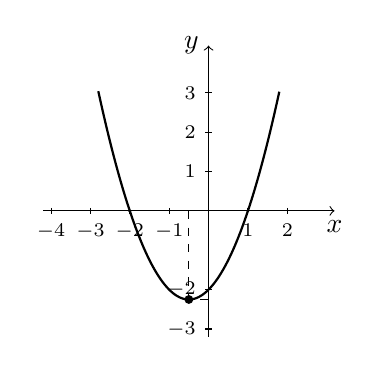
\begin{tikzpicture}[scale=0.5]
    \draw[->] (-4.2,0) -- (3.2,0) node[below] {$x$};
    \draw[->] (0,-3.2) -- (0,4.2) node[left] {$y$};
    \foreach \x in {-4,-3,-2,-1,1,2}
        \draw (\x,0.08) -- (\x,-0.08) node[below] {\scriptsize $\x$};
    \foreach \y in {-3,-2,1,2,3}
        \draw (0.08,\y) -- (-0.08,\y) node[left] {\scriptsize $\y$};
    \draw[smooth, samples=200, domain=-2.8:1.8, thick] plot (\x, {\x*\x+\x-2});
    \fill (-2,0) circle (1.2pt);
    \fill (1,0) circle (1.2pt);
    \fill (-0.5,-2.25) circle (3.2pt);
    \draw[dashed] (-0.5,0) -- (-0.5,-2.25);
    \draw[dashed] (0,-2.25) -- (-0.5,-2.25);
\end{tikzpicture}

\end{center}
Tập nghiệm của bất phương trình $f\left(x\right)\ge 0$ là
\ChoicesOneLine
{$\left[-2;1\right]$.}
{$\left(-\infty;-2\right]\cup\left[1;+\infty\right)$.}
{$\left(-2;1\right)$.}
{$\left(-\infty;-2\right)\cup\left(1;+\infty\right)$.}
{2}
\SolutionBlock{Từ đồ thị, parabol mở lên và cắt trục hoành tại $x=-2$ và $x=1$. Vì vậy $f\left(x\right)\ge0$ khi $x\le -2$ hoặc $x\ge1$, tức là $\left(-\infty;-2\right]\cup\left[1;+\infty\right)$.}

\NQuestion Tập nghiệm của bất phương trình $2x^2-7x+3<0$ là
\ChoicesOneLine
{$\left(\dfrac12;3\right)$.}
{$\left(-\infty;\dfrac12\right)\cup\left(3;+\infty\right)$.}
{$\left[\dfrac12;3\right]$.}
{$\left(-\infty;\dfrac12\right]\cup\left[3;+\infty\right)$.}
{1}
\SolutionBlock{Ta có $2x^2-7x+3=(2x-1)(x-3)$. 
\\Vì hệ số $a=2>0$ nên tam thức âm giữa hai nghiệm phân biệt $\dfrac12$ và $3$. 
\\Vậy tập nghiệm là $\left(\dfrac12;3\right)$.}

\NQuestion Phương trình $\sqrt{x^2-5x+6}=x-2$ có nghiệm là
\ChoicesOneLine
{$x=2$.}
{$x=3$.}
{$x=2$ hoặc $x=3$.}
{Phương trình vô nghiệm.}
{1}
\SolutionBlock{Điều kiện: $x-2\ge0\Leftrightarrow x\ge2$. Bình phương hai vế:
\[
x^2-5x+6=(x-2)^2=x^2-4x+4 \Rightarrow -x+2=0 \Rightarrow x=2.
\]
Thử lại vào phương trình ban đầu: $\sqrt{4-10+6}=0=x-2$. Vậy nghiệm duy nhất là $x=2$.}

\NQuestion Một mật khẩu gồm $1$ chữ cái in hoa tiếng Anh theo sau bởi $3$ chữ số khác nhau. Số mật khẩu có thể tạo thành là
\ChoicesOneLine{$26\cdot 10^3$.}{$26\cdot A_{10}^3$.}{$26\cdot C_{10}^3$.}{$A_{26}^4$.}{2}
\SolutionBlock{Có $26$ cách chọn chữ cái đầu tiên. Ba chữ số khác nhau xếp theo thứ tự nên có $A_{10}^3=10\cdot9\cdot8$ cách. Theo quy tắc nhân, số mật khẩu là $26\cdot A_{10}^3$.}

\NQuestion Có bao nhiêu cách xếp $7$ học sinh phân biệt thành một hàng ngang nếu hai bạn An và Bình luôn đứng cạnh nhau?
\ChoicesOneLine{$7!$.}{$2\cdot 6!$.}{$2\cdot 5!$.}{$6!$.}{2}
\SolutionBlock{Xem cặp An, Bình như một khối. Khi đó có $6$ đối tượng cần sắp xếp nên có $6!$ cách. Trong mỗi cách, An và Bình có thể đổi chỗ cho nhau theo $2!$ cách. Vậy có $2\cdot6!$ cách.}

\NQuestion Từ các chữ số $0,1,2,3,4,5,6$, lập được bao nhiêu số tự nhiên có $4$ chữ số khác nhau và chia hết cho $5$?
\ChoicesOneLine{$200$.}{$220$.}{$216$.}{$240$.}{2}
\SolutionBlock{Số chia hết cho $5$ nên chữ số hàng đơn vị là $0$ hoặc $5$.
\begin{itemize}[leftmargin=1.5em]
\item Nếu hàng đơn vị là $0$: hàng nghìn có $6$ cách chọn ($1$ đến $6$), hàng trăm có $5$ cách, hàng chục có $4$ cách. Có $6\cdot5\cdot4=120$ số.
\item Nếu hàng đơn vị là $5$: hàng nghìn không được là $0$ hay $5$, nên có $5$ cách. Hàng trăm có $5$ cách, hàng chục có $4$ cách. Có $5\cdot5\cdot4=100$ số.
\end{itemize}
Tổng cộng có $120+100=220$ số.}

\NQuestion Trong mặt phẳng tọa độ $Oxy$, cho $A(2;-1)$ và $B(-3;4)$. Tọa độ vectơ $\overrightarrow{BA}$ là
\ChoicesOneLine{$(-5;5)$.}{$(5;-5)$.}{$(-1;3)$.}{$(1;-3)$.}{2}
\SolutionBlock{Ta có $\overrightarrow{BA}=(2-(-3);\,-1-4)=(5;-5)$.}

\NQuestion Trong mặt phẳng tọa độ $Oxy$, cho tam giác $ABC$ với $A(1;2)$, $B(5;0)$, $C(-2;4)$. Tọa độ trọng tâm $G$ là
\ChoicesOneLine
{$\left(\dfrac43;2\right)$.}
{$\left(1;2\right)$.}
{$\left(\dfrac43;\dfrac83\right)$.}
{$\left(2;2\right)$.}
{1}
\SolutionBlock{Ta có
\[
G\left(\dfrac{1+5+(-2)}{3};\dfrac{2+0+4}{3}\right)=\left(\dfrac43;2\right).
\]}

\NQuestion Đường thẳng đi qua $M(1;3)$ và nhận vectơ pháp tuyến $\vec n=(2;-1)$ làm vectơ pháp tuyến có phương trình là
\ChoicesOneLine
{$2x-y+1=0$.}
{$2x-y-1=0$.}
{$x+2y-7=0$.}
{$x-2y+5=0$.}
{1}
\SolutionBlock{Đường thẳng có dạng $2x-y+c=0$. Thay $M(1;3)$ vào:
\[
2\cdot1-3+c=0 \Rightarrow c=1.
\]
Suy ra phương trình là $2x-y+1=0$.}

\NQuestion Cho đồ thị hàm số $y=f\left(x\right)$ như hình vẽ dưới đây.
\begin{center}
    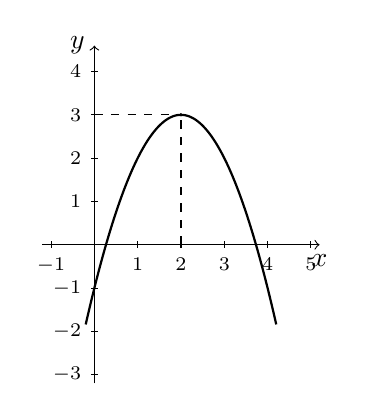
\begin{tikzpicture}[scale=0.55]
    \draw[->] (-1.2,0) -- (5.2,0) node[below] {$x$};
    \draw[->] (0,-3.2) -- (0,4.6) node[left] {$y$};
    \foreach \x in {-1,1,2,3,4,5}
        \draw (\x,0.08) -- (\x,-0.08) node[below] {\scriptsize $\x$};
    \foreach \y in {-3,-2,-1,1,2,3,4}
        \draw (0.08,\y) -- (-0.08,\y) node[left] {\scriptsize $\y$};
    \draw[smooth, samples=200, domain=-0.2:4.2, thick] plot (\x, {-(\x-2)^2+3});
    \fill (2,3) circle (1.2pt);
    \draw[dashed] (2,0) -- (2,3);
    \draw[dashed] (0,3) -- (2,3);
\end{tikzpicture}

\end{center}
Số nghiệm của phương trình $f\left(x\right)=1$ là
\ChoicesOneLine{$0$.}{$1$.}{$2$.}{$3$.}{3}
\SolutionBlock{Đường thẳng $y=1$ cắt parabol mở xuống tại hai điểm phân biệt. Vì đỉnh có tung độ lớn hơn $1$, nên phương trình $f\left(x\right)=1$ có $2$ nghiệm phân biệt.}

\NQuestion Gọi $\alpha$ là góc giữa hai đường thẳng $d_1:x-2y+3=0$, $d_2:2x+y-4=0$.
Khi đó
\ChoicesOneLine
{$\alpha=30^\circ$.}
{$\alpha=45^\circ$.}
{$\alpha=60^\circ$.}
{$\alpha=90^\circ$.}
{4}
\SolutionBlock{Ta có $d_1:y=\dfrac12x+\dfrac32$ nên $m_1=\dfrac12$, còn $d_2:y=-2x+4$ nên $m_2=-2$. Vì $m_1m_2=-1$ nên hai đường thẳng vuông góc nhau. Do đó $\alpha=90^\circ$.}

\NQuestion Khoảng cách từ điểm $P\left(3;-1\right)$ đến đường thẳng $d:2x-y+4=0$ bằng
\ChoicesOneLine
{$\dfrac9{\sqrt5}$.}
{$\dfrac{11}{\sqrt5}$.}
{$\sqrt5$.}
{$\dfrac7{\sqrt5}$.}
{2}
\SolutionBlock{Ta có
\[
d(P,d)=\dfrac{|2\cdot3-(-1)+4|}{\sqrt{2^2+(-1)^2}}=\dfrac{11}{\sqrt5}.
\]}
